\section{Preliminaries}
\label{prelimiary}
While there are many existing protocols designed for specific scenarios and they focus on preserving different properties with various trust base. \dprotocol targets to achieve liveness, safety, permissionless, and linearizability properties by using zero-knowledge proof to provide a universal layer that synchronizes states between different smart contracts on different blockchains, and this layer together with its communication protocol can be used as a multi-blockchain communication framework. Below we first briefly review several key concepts in our protocol and then describe the main idea behind \dprotocol. For a detailed description of these concepts, we refer to \cite{robinson2021survey}. 

\smallskip\noindent\textbf{Blockchain.}
A blockchain is a distributed database that is shared among a network of distributed nodes \cite{chen2018survey}. As a database, transactions are first submitted and organized in blocks, while each block is a data structure that records the most recent transactions which have not yet been validated. Once a block is validated, the state of the whole distributed database is updated accordingly.

\smallskip\noindent\textbf{Bundled multi-blockchain Transaction.}
We use $C$ (with possible subscripts) to denote a particular blockchain system with distributed nodes. For a blockchain $C_k$ indexed with $k$, We use $S_k$ to denote the whole state of a blockchain $C_{k}$ and $s_k$ to describe a \emph{partial} state in $S_k$.

Given a group of blockchains $C_{1}, C_{2}, \cdots, C_{k}$, we say a transaction $tx$ is a bundled multi-blockchain transaction if it is composed of a sequence of transactions $tx_{k_0}^0$, $tx_{k_1}^1$, $\cdots$ $tx_{k_j}^j$ such that the $j$th involved sub-transaction $tx_{k_j}^j$ is supposed to be executed on $C_{k_j}$ locally and the behavior of each $tx_{k_j}^{j}$ depends on state $s_{k_j}$. 

In a bundled transaction $tx$, We use $s= \langle s_1, s_2, \cdots, s_k \rangle$ to denote the underlying global state of $tx$ where $s_k$ denotes the projection of $s$ on the blockchain $C_k$. Moreover each local transaction $tx_k^j$ is executed on the partial state of $s_k$ in $C_k$. For example, a bundled transaction could look like the following. 
\begin{lstlisting}[escapeinside={(*}{*)}, backgroundcolor = \color{white}, basicstyle=\small,]
(*$tx(s)$*){
    (*$s^1 = \langle tx_0(s_0^0), s_1^0, s_2^0, \cdots \rangle$*)
    (*$s^2 = \langle s_0^1, tx_1(s_1^1), s_2^1, \cdots \rangle$*)
    ....
    (*$s^n = \langle s_0^{n-1}, s_1^{n-1}, s_2^{n-1}, tx_n(s_{k}^{n-1})\rangle$*)
}
\end{lstlisting}
where $tx_0$ is performed on local state $s_0$, $tx_1$ is performed on local state $s_1$ ..., and the global state $s$ is changed to $s^n$ after $tx$ is fully performed.

\smallskip\noindent\textbf{Aggregator Chain.}
In this work, we will introduce an extra blockchain to store the global state $s$. We denote this chain as an \emph{aggregator chain} to distinguish it from other blockchains $C_{k}$ involved in a bundled multi-blockchain transaction $tx$. Moreover, we call the other blockchains \emph{native chains}.

\smallskip\noindent\textbf{Merkle Tree Encoding of a Global State.}
Merkle tree \cite{becker2008merkle} is a tree (see Figure \ref{merkle-tree}) in which every leaf node is labeled with the cryptographic hash ($P = hash(leaves)$) of a data block, and every non-leaf node is labeled with the cryptographic hash of the labels of its child nodes. Each data block has a unique Merkle tree index (MTI) and each MTI encodes a unique path from top to leaf.\\

\begin{figure}[!ht]
\centerline{
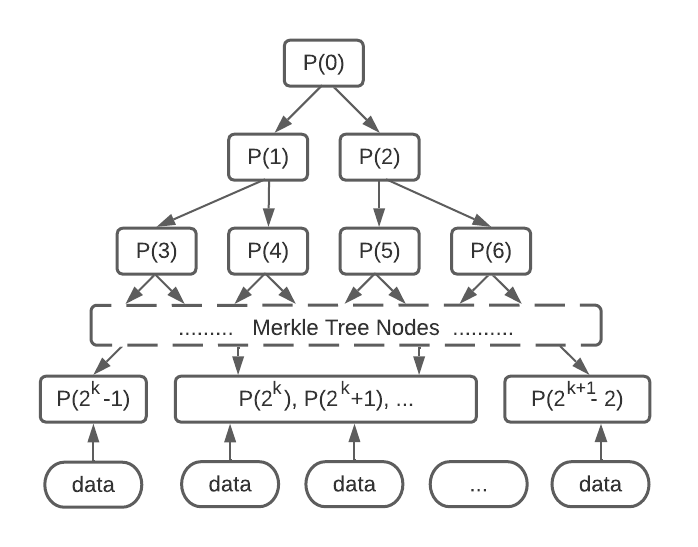
\includegraphics[scale=0.6]{merkle-tree}}
\caption{Merkle tree structure}\label{merkle-tree}
\end{figure}

\smallskip\noindent\textbf{State Pinning.}
State Pinning \cite {robinson2019anonymous} is defined as including the state of one blockchain in another blockchain. In our scenario, we encode our global state into the Merkle tree and use the Merkle root hash to pin the global state in native blockchains to ensure that the global state used in the simulation of transactions is consistent.

\smallskip\noindent\textbf{Side Effect.}
We denote the changes of $tx_i^k$ on chain-state $C_k$ other than the partial state $s_k$ to be the side effect $e_k$ of of $tx_i^k$. Side effects can be emitting events on native chains or native chain contract calls.

\smallskip\noindent\textbf{Polynomial Commitment Schemes.}
Polynomial commitment schemes (PCS) \cite{boneh2020halo-pcs,boneh2020efficient-pcs,kate2010polynomial-pcs} provides the ability to commit to a polynomial over a finite field and prove its evaluation at points. A succinct PCS has commitment and evaluation proof size sublinear in the degree of the polynomial. An efficient PCS has sublinear proof verification. Any efficient and succinct PCS can be used to construct a SNARK \cite{mayer2016zk} with similar security and efficiency characteristics.

\smallskip\noindent\textbf{Zero Knowledge Proof of Program Execution.}
Since PCS provides a scheme to prove the evaluation of polynomials at certain points, we can convert program evaluation into polynomial equations so that the problem of proving a program has certain results can be converted into problems of polynomial equations. Furthermore, a zero-knowledge proof \cite{cramer1998zero-zkp,kate2010constant-zkp,damgaard1998commitment-zkp} of program execution is a PCS proof that can be used by a prover to convince a verifier that a program is executed correctly without leaking any private information.

%\smallskip In the next section, we present a brief picture of our solution by a case study (see Section \ref{chp:case-study}) of the standard transfer and explain how zero knowledge is applied so that the safety, liveness, and permissionless properties hold. In Section \ref{chp:protocol-details} we describe each component in detail and then we explain the trust base of our solution and prove that under the trust base our solution has a full guarantee of safety, permissionless and liveness properties (see Section \ref{chp:properities}).

%Regarding the permissionless, we need to ensure that neither safety and liveness properties can be affected when introducing new decentralized nodes in \dprotocol. Since safety is enforced by ZKP(zero-knowledge proof), it is sufficient to prevent newly joined nodes from ordering transactions unfairly. Therefore we use BFT(Byzantine Fault Tolerant) consensus algorithm and permissionless property relies on that two-thirds of the nodes of the aggregator chain are honest.